\section{Raffinamento del Modello di Dominio}\label{sec:raffmoddom}

\subsection{Premesse}
In seguito ai primi suggerimenti forniti nella Sezione \vref{subsubsec:aamddomsugg_admin},
si è iniziato a ristrutturare il modello di dominio. 
\begin{itemize}
\item Per quanto concerne lo ``Slot'' orario indicato nella nostra precedente
	visualizzazione, questo sarà un'astrazione delle informazioni di data, ora e
	prenotazione già presente all'interno come campi di \texttt{Prenotazione}
\end{itemize}


\subsubsection{Strutturazione dei campi Messaggio}
Dopo aver ribadito che ``una richiesta di prenotazione (inviata appunto tramite
messaggio) non è ancora una prenotazione'' (la quale sarà di un tipo di dato
\texttt{Prenotazione}), procediamo ad analizzare 
i campi necessari per le due tipologie di messaggi,
poiché dobbiamo poter modellare le nostre classi \texttt{MAmministratore} e
\texttt{MPaziente}, i quali rappresentano rispettivamente i messaggi inviati
dagli amministratori e quelli inviati dai pazienti, possiamo fare le seguenti
considerazioni:
\begin{itemize}
\item Anche se sarebbe possibile distinguere per ogni tipo di messaggio, \texttt{MPaziente}
	ed \texttt{MAmministratore} tra tipologie di \textit{prenotazione}, \textit{posticipo} e
	\textit{cancellazione} ed analoghe conferme lato amministratore, preferiamo
	mantenere distinti i valori come analizzato nel primo Documento
	dell'Architettura software pubblicato (v. Sezione \vref{sec:docarchsoft}).
	Il tipo della richiesta o della notifica viene quindi specificato nel 
	campo $kind$ del messaggio.
\end{itemize}
\begin{description}
\item[MPaziente]
Per i messaggi paziente, possiamo sottolineare che:
\begin{itemize}
\diam I messaggi per l'amministratore costituiscono le richieste (es. di prenotazione) che
	devono essere gestite dagli amministratori: una volta che queste
	sono state gestite, il sistema provvederà in automatico a rimuoverle
	dal sistema.
\diam Per revocare, annullare o posticipare la visita, non è richiesto
	l'inserimento di testo.
\diam Unicamente per effettuare una richiesta di prenotazione, non è necessario
	associare al messaggio una prenotazione, in quanto questa deve essere
	ancora creata dall'Amministratore. Negli altri due casi di richiesta
	è invece necessaria, in quanto bisogna specificare su quale richiesta
	si stia facendo l'interrogazione.
\diam L'inserimento di una descrizione è necessaria unicamente nella descrizione
	della richiesta lato amministratore.
\diam Il mittente è il paziente che effettua la richiesta.
\diam Il destinatario è l'amministratore responsabile della gestione dei
	messaggi per quel reparto nel quale l'utente chiede di essere visitato.
\end{itemize}

\item[MAmministratore]
Per i messaggi amministratore, possiamo sottolineare che questi verranno
generati automaticamente dall'interazione dello stesso con l'interfaccia grafica:
\begin{itemize}
\diam Per notificare la revoca di una prenotazione, è necessario utilizzare
	il campo testo, in quanto è comunque necessario memorizzare le 
	informazioni di una prenotazione che è stata rimossa.
\diam Il mittente è l'amministratore che sta effettuando la risposta.
\diam Il destinatario è il paziente che riceverà la notifica.
\diam Unicamente nell'invio di una notifica di cancellazione, è richiesto
	specificare la prenotazione che è stata cancellata: negli altri casi
	questo campo è di per se inutilizzato, e lasciato per eventuali estensioni.
\end{itemize}
\end{description}

Ulteriori dettagli sulla definizione degli attributi necessari alle classi,
sono forniti all'interno dell'Analisi Logica del Database (v. \vref{sec:proglogicadb}).

\subsubsection{Implicazioni dell'utilizzo del framework ``EJP''}
Possiamo sottolineare che l'utilizzo di un \textit{framework per la persistenza}
come EJP\footnote{Easy Java Persistence: \texttt{http://www.easierjava.com/}}, 
di cui parleremo dettagliatamente  nella Sezione \vref{sec:dbutilizzejp},
possa effettivamente demandare la gestione della rappresentazione delle singole
classi al framework: conseguentemente all'applicazione di un design pattern \textit{Singleton}
per l'accesso al database in questo contesto, non si ha conseguentemente alcun
incremento di
responsabilità nella gestione del cambiamento delle classi. Questo framework
infatti si occupa automaticamente di effettuare il mapping tra modelli $OO$ e $ER$.


\subsubsection{Applicazione di design pattern}\label{subsubsec:applydesignpatt}
In seconda analisi, possiamo passare all'applicazione dei design pattern all'interno
di questo contesto.

\begin{description}
\item[Factory Method] Abbiamo applicato questo design pattern per effettuare 
	il ``login'' dei pazienti e per effettuare la loro creazione: tuttavia
	se dovessimo applicare il \textbf{Single Responsability Principle} in
	questo contesto, dovremmo dividere il ``login'' dalla loro registrazione,
	in quanto sono due aspetti differenti dello stesso problema. Tuttavia,
	in questo modo, si rischierebbe di riprodurre tre volte questa gerarchia:
	una per la definizione dei dati da creare (5 classi), ed altre due 
	per definire le Factory di autenticazione e di creazione: preferiamo
	per tanto tenere unite queste responsabilità. L'elemento radice della
	\textit{Factory} è \texttt{GuestC}. 
	
	Si vuole inoltre sottolineare come i metodi
	ivi definiti $login$ e $create$ siano stati inseriti puramente per sottolineare
	la necessità di riflettere anche quivi la gerarchia imposta per gli utenti.
\item[Facade] Per effettuare la visualizzazione delle prenotazioni e dei referti,
	abbiamo identificato la classe \texttt{ViewSupport} allo scopo di riunire
	le diverse logiche di visualizzazione implementate. 
\item[Singleton] Per garantire \textbf{Hight Cohesion}, allo scopo di fornire un
	accesso al database in un unico punto dell'applicazione, .
\end{description}
\bigskip

Dopo queste ultime valutazioni, possiamo effettuare una prima revisione del
Modello di Dominio, come presentato in Figura \vref{fig:firstdmrevision}.

\begin{figure}[p]
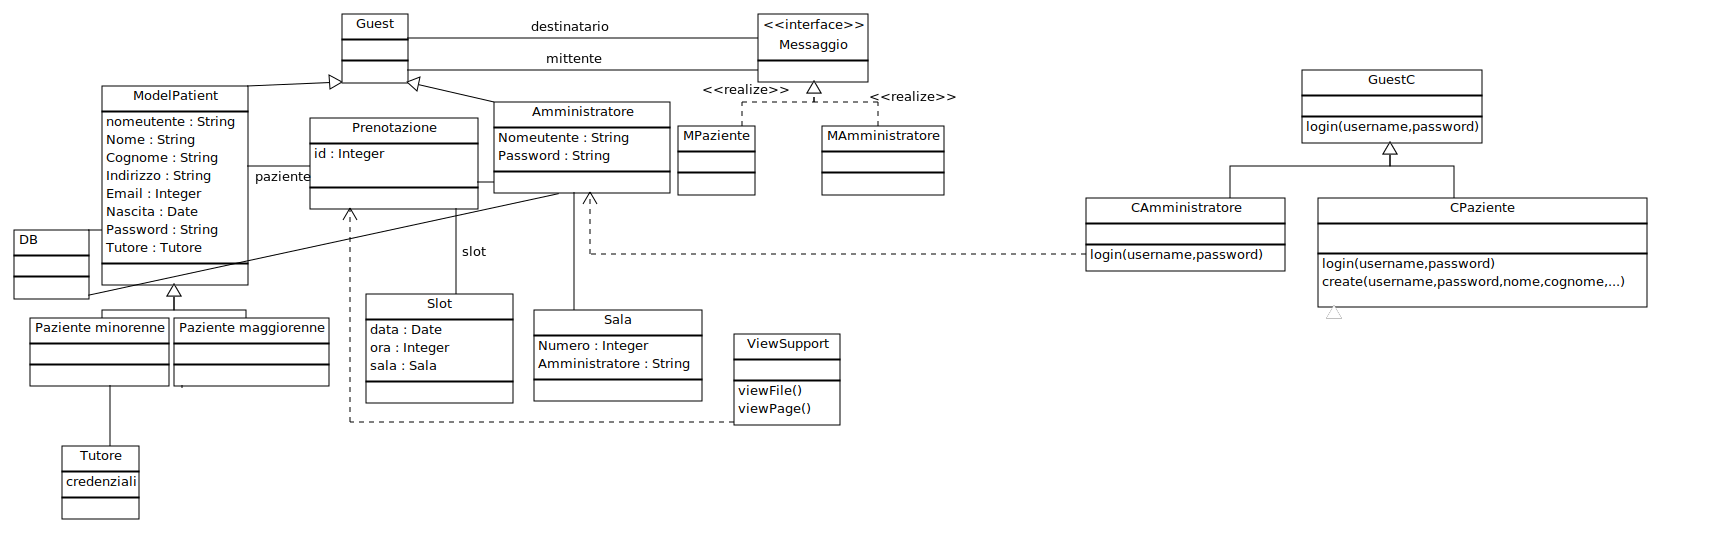
\includegraphics[scale=0.5,angle=90]{svgs2/DomainModel01}
\caption{\textit{First Revision of the Domain Model presented in Section \vref{sec:domainmodel}}.}
\label{fig:firstdmrevision}
\end{figure} 
